%!TEX root = ../../../../exa-ma-d7.1.tex

\section{Compute distance to a range of entities}


\Cref{tab:app-feelpp-distance} describes the specifications of the application.

\begin{table}[ht]
    \centering
    \begin{tblr}{
        colspec = {l X[10cm]},
        row{odd} = {numpexlightergray},
        hlines = {0.1pt, numpexgray},
        vlines = {numpexgray},
        row{1} = {numpexgray, fg=white, font=\bfseries},
    }
        Field & Details \\
        id & \texttt{app-feelpp-distance} \\
        name & Distance \\
        Partners & Unistra \\
        PC & PC1 - ExaMA, PC2 - ExaSoft \\
        Responsible (Permanent) & V. Chabannes; C. Prud'homme \\
        WP7 Engineer & Thomas Saigre (UNISTRA) \\
        work\_package & WP1 \\
        application\_type & mini-app \\
        purpose & Compute distance to a range of entities using FMM or BVH \\
        Method-Algorithm WP1 &  unstructured mesh, finite element, FMM, ray-tracing-BVH \\
        Method-Algorithm WP2 & \\
        Method-Algorithm WP3 & \\
        Method-Algorithm WP4 & \\
        Method-Algorithm WP5 & \\
        Method-Algorithm WP6 & \\
        WP7 & \\
        % inputs &  \\
        % outputs & \\
        % metrics & \\
        % status & \\
        % Benchmark scope & \\
        % Framework & \\
        % parallel\_framework & \\
        % spec\_due & \\
        % proto\_due & \\
        repo\_url & \url{https://github.com/numpex/apps-feelpp}\\
    \end{tblr}
    \caption{Description of the mini-app \texttt{app-feelpp-distance}.}
    \label{tab:app-feelpp-distance}
\end{table}


%%%%%%%%%%%%%%%%%%%%%%%%%%%%%%%%%%%%%%%%%%%%%%%%%%%%%%%%%%%%%%%%%%%%%%%%%%%%%%%%%%%%%%%%%%%%%%%%%%%%%%%%%%%%%%%%%%%%%%%%


\subsection{Description of the benchmark}

We consider the unit cube $[0,1]^3$ discretized by an unstructured tetrahedral mesh.
Let $h$ denote the mesh size, controlling the total number of vertices $N$.
For each mesh vertex $\mathbf{x}_i$, our goal is to compute the Euclidean distance
\begin{equation}\label{eq:distance-definition}
  d(\mathbf{x}_i) = \min_{\mathbf{y}\in\partial([0,1]^3)} \Vert\mathbf{x}_i - \mathbf{y}\Vert_2.
\end{equation}
The exact analytical distance on the unit cube is
\begin{equation}\label{eq:distance-exact}
  d_{\mathrm{exact}}(x,y,z) = \min\{x,\,1-x,\,y,\,1-y,\,z,\,1-z\}.
\end{equation}
We compare two numerical strategies to build a continuous piecewise-linear (P1) distance field over the mesh.

More details can be found in \cite{van_landeghem_micro-swimming_2025}.


\subsubsection{Fast--Marching Method (FMM)}
\begin{enumerate}
  \item \textbf{Initialization:} Tag all boundary vertices of the mesh as known with $d=0$.
  \item \textbf{Propagation:} Maintain a narrowband of trial vertices adjacent to known ones. Repeatedly extract the trial vertex with the minimal tentative distance, mark it known, and update neighboring trial vertices by solving local upwind discretization of the eikonal equation $\Vert\nabla d\Vert = 1$.
  \item \textbf{Output:} A P1 scalar field $d_h(\mathbf{x})$ approximating the true distance.
\end{enumerate}

\subsubsection{Ray-Tracing with BVH}
\begin{enumerate}
  \item \textbf{Preprocessing:} Build a Bounding Volume Hierarchy (BVH) over the mesh boundary faces or directly on the analytic cube faces.
  \item \textbf{Directional Sampling:} Since the cube geometry is known, but the nearest boundary direction is unknown, for each vertex $\mathbf{x}_i$ we uniformly sample directions on the unit sphere. Let $M$ be the number of rays per point, which becomes a key parameter for accuracy and cost.
  \item \textbf{Ray Casting:} For each sampled direction, cast a ray from $\mathbf{x}_i$ into the BVH and record the intersection distance. The estimated distance is the minimum over all sampled rays:
  \[ d_h(\mathbf{x}_i) = \min_{1\le j\le M} t_j, \]
  where $t_j$ is the distance along ray $j$ to the boundary.
  \item \textbf{Output:} A P1 field $d_h(\mathbf{x})$ by assigning the computed distance at each vertex.
\end{enumerate}



%%%%%%%%%%%%%%%%%%%%%%%%%%%%%%%%%%%%%%%%%%%%%%%%%%%%%%%%%%%%%%%%%%%%%%%%%%%%%%%%%%%%%%%%%%%%%%%%%%%%%%%%%%%%%%%%%%%%%%%%


\subsection{Benchmarking tools used}

Let $d_h$ be the discrete distance field computed by either method. We compute the error norms
\begin{subequations}
\begin{align}
  \Vert d_h - d_{\mathrm{exact}}\Vert_{L^2} &= \left( \sum_{i=1}^N (d_h(\mathbf{x}_i) - d_{\mathrm{exact}}(\mathbf{x}_i))^2
    \right)^{1/2},\\
  \Vert d_h - d_{\mathrm{exact}}\Vert_{L^\infty} &= \max_{i=1,\dots,N} |d_h(\mathbf{x}_i) - d_{\mathrm{exact}}(\mathbf{x}_i)|.
\end{align}
\label{eq:specs:feelpp:distance:error}
\end{subequations}

We perform a convergence study over meshes with $h = h_0, h_0/2, h_0/4, \dots$, verifying that FMM yields $O(h)$ convergence, while ray-tracing achieves machine-precision at vertices.



%%%%%%%%%%%%%%%%%%%%%%%%%%%%%%%%%%%%%%%%%%%%%%%%%%%%%%%%%%%%%%%%%%%%%%%%%%%%%%%%%%%%%%%%%%%%%%%%%%%%%%%%%%%%%%%%%%%%%%%%


\subsection{Input/Output Dataset Description}


\subsubsection{Input Data:}
  \begin{itemize}
  \item Meshes: we use a cubic mesh with a various discretization size: $h = 0.12, 0.06, 0.03$ and $0.015$.
  \item Setup: the FMM method is provided by the core library of \Feelpp, and the BVH implementation uses functionalities of \Feelpp.
    More details can be found in \cite{van_landeghem_micro-swimming_2025}.
  \end{itemize}


\subsubsection{Output Data:}

The output data monitored are the $L^2$ error committed by the two methods on the benchmark, as described in \Cref{eq:specs:feelpp:distance:error},
as well as the time of execution to compute the distance for all points $\mathbf{x}_i$ in the mesh.


%%%%%%%%%%%%%%%%%%%%%%%%%%%%%%%%%%%%%%%%%%%%%%%%%%%%%%%%%%%%%%%%%%%%%%%%%%%%%%%%%%%%%%%%%%%%%%%%%%%%%%%%%%%%%%%%%%%%%%%%

\subsection{Results summary}

We present in this section the results of the benchmark described above.
In \Cref{fig:specs:app-feelpp-distance:results:distance}, we show the exact distance between each point of the cube to the border.
The cube is vertically half sliced.

We also present in \Cref{fig:specs:app-feelpp-distance:results:error-bvh} and \Cref{fig:specs:app-feelpp-distance:results:error-bvh} respectively the distribution of the point wise error for the methods FMM and BVH respectively.
For this specific plot, we took $h=0.06$ and $M=1500$.
We note that the BVH method results in a smaller global error, while it is more localized for the FMM method.


\begin{figure}
    \begin{subfigure}{0.33\textwidth}
        \centering
        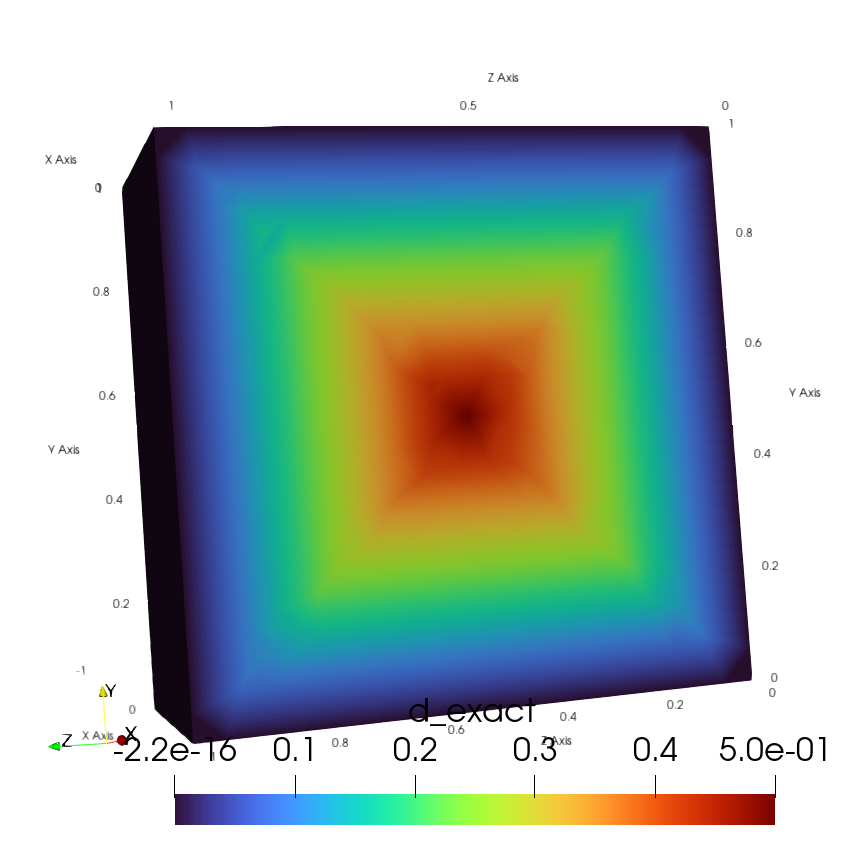
\includegraphics[width=\columnwidth]{graphics/feelpp/feelpp-benchmark-distance-exact}
        \caption{Exact distance $d_\mathrm{exact}$.}
        \label{fig:specs:app-feelpp-distance:results:distance}
    \end{subfigure}
    \begin{subfigure}{0.33\textwidth}
        \centering
        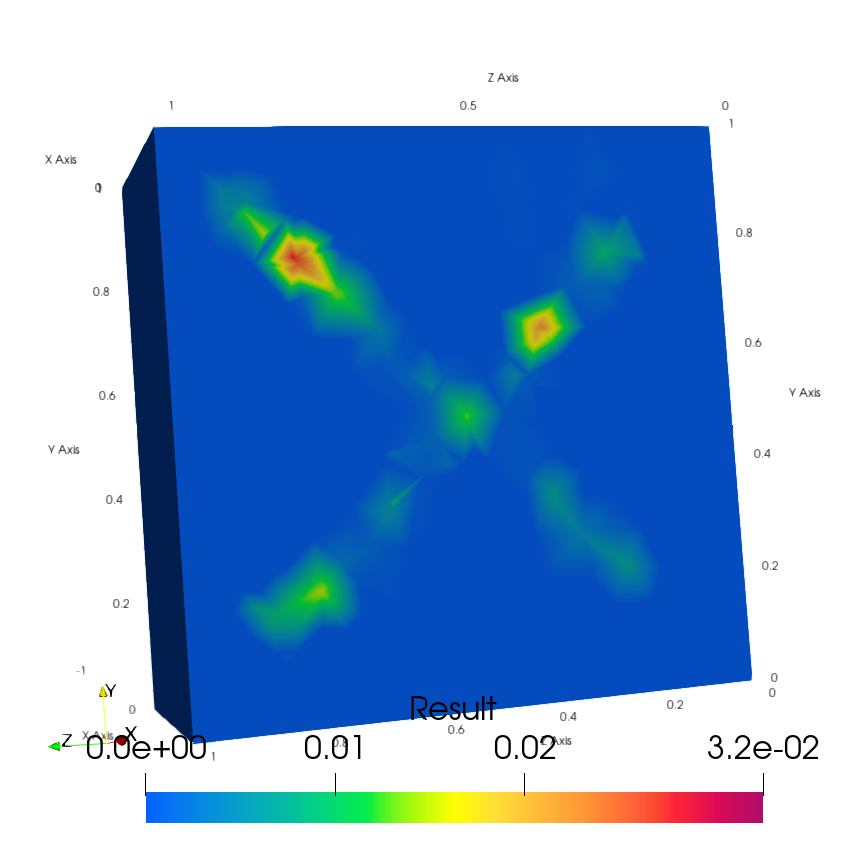
\includegraphics[width=\columnwidth]{graphics/feelpp/feelpp-benchmark-distance-errorFMM}
        \caption{Error by the method FMM: $|d_\mathrm{FMM}-d_\mathrm{exact}|$.}
        \label{fig:specs:app-feelpp-distance:results:error-fmm}
    \end{subfigure}
    \begin{subfigure}{0.33\textwidth}
        \centering
        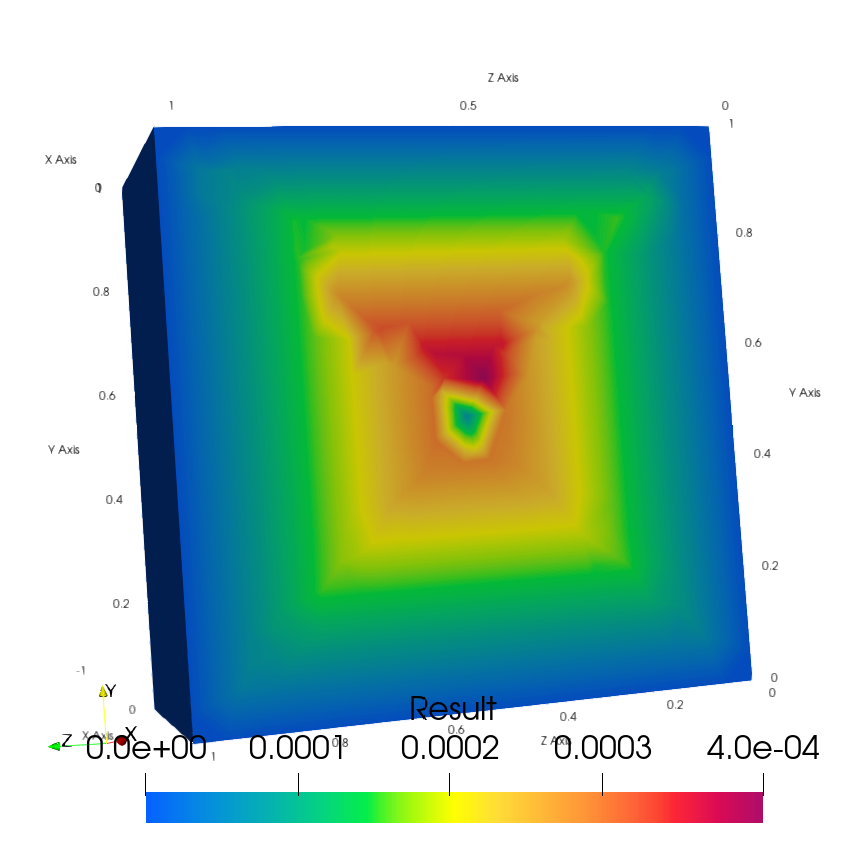
\includegraphics[width=\columnwidth]{graphics/feelpp/feelpp-benchmark-distance-errorBVH}
        \caption{Error by the method BVH: $|d_\mathrm{BVH}-d_\mathrm{exact}|$.}
        \label{fig:specs:app-feelpp-distance:results:error-bvh}
    \end{subfigure}
    \caption{Numerical results of distance computing, with $h=0.06$ and $M=1500$.}
    \label{fig:specs:app-feelpp-distance:results}
\end{figure}

We now present some results of convergence.
Note that for some cases, such as high meshes or high number of ray cast, the BVH method did not finish as it require too much memory.


\pgfplotstableread[col sep=comma]{chapters/applications/specs/data/app-feelpp-distance/timeBVH1000.csv}\dataTimeBVHnp
\pgfplotstableread[col sep=comma]{chapters/applications/specs/data/app-feelpp-distance/speedupBVH1000.csv}\dataSpeedupBVHnp
\pgfplotstableread[col sep=comma]{chapters/applications/specs/data/app-feelpp-distance/timeFMM1000.csv}\dataTimeFMMnp
\pgfplotstableread[col sep=comma]{chapters/applications/specs/data/app-feelpp-distance/speedupFMM1000.csv}\dataSpeedupFMMnp
\pgfplotstableread[col sep=comma]{chapters/applications/specs/data/app-feelpp-distance/errorBVHRay.csv}\dataTimeBVHM
\pgfplotstableread[col sep=comma]{chapters/applications/specs/data/app-feelpp-distance/convergenceBVH.csv}\dataConvBVH
\pgfplotstableread[col sep=comma]{chapters/applications/specs/data/app-feelpp-distance/convergenceFMM.csv}\dataConvFMM


\begin{figure}
  \centering
  \begin{subfigure}{0.49\textwidth}
    \begin{tikzpicture}
    \begin{axis}[
      width=\textwidth,
      xlabel={ Number of tasks }, ylabel={ Time [s] },
      xtick=data, xtick align=outside,
      ymode=log,
      ymajorgrids=true, yminorgrids=true,
      xmajorgrids=true,
      xticklabels from table={\dataTimeBVHnp}{tasks},
      cycle list name=color list, legend style={at={(0.99, 0.01)},anchor=south east}
    ]
      \addplot+[mark=*, color=customdarkblue] table [x expr=\coordindex, y=0.12] {\dataTimeBVHnp} ;
      % \addlegendentry{ $h=0.12$ }
      \addplot+[mark=*, color=customcyan] table [x expr=\coordindex, y=0.06] {\dataTimeBVHnp} ;
      % \addlegendentry{ $h=0.06$ }
      \addplot+[mark=diamond*, dashed, color=customdarkblue, forget plot] table [x expr=\coordindex, y=0.12] {\dataTimeFMMnp} ;
      \addplot+[mark=diamond*, dashed, color=customcyan, forget plot] table [x expr=\coordindex, y=0.06] {\dataTimeFMMnp} ;
    \end{axis}
    \end{tikzpicture}
    \caption{Evolution of the time for the methods BVH and FMM depending on the number of parallel process. }
    \label{fig:app:feelpp-distance:results:np}
  \end{subfigure}
  \begin{subfigure}{0.49\textwidth}
    \begin{tikzpicture}
    \begin{axis}[
      width=\textwidth,
      xlabel={ Number of tasks }, ylabel={ Time [s] },
      xtick=data, xtick align=outside,
      ymode=log,
      ymajorgrids=true, yminorgrids=true,
      xmajorgrids=true,
      xticklabels from table={\dataSpeedupBVHnp}{tasks},
      cycle list name=color list, legend style={at={(0.01, 0.01)},anchor=south west}
    ]
      \addplot+[mark=*, color=customdarkblue] table [x expr=\coordindex, y=0.12] {\dataSpeedupBVHnp} ;
      \addlegendentry{ $h=0.12$ }
      \addplot+[mark=*, color=customcyan] table [x expr=\coordindex, y=0.06] {\dataSpeedupBVHnp} ;
      \addlegendentry{ $h=0.06$ }
      \addplot+[mark=diamond*, dashed, color=customdarkblue, forget plot] table [x expr=\coordindex, y=0.12] {\dataSpeedupFMMnp} ;
      \addplot+[mark=diamond*, dashed, color=customcyan, forget plot] table [x expr=\coordindex, y=0.06] {\dataSpeedupFMMnp} ;
      % \addplot+[mark=none, dashed, color=black] table [x expr=\coordindex, y=optimal] {\dataSpeedupBVHnp} ;
      % \addlegendentry{Optimal}
    \end{axis}
    \end{tikzpicture}
    \caption{Comparison of speedup for BVH and FMM. }
    \label{fig:app:feelpp-distance:results:speedup}
    \vspace{0.8\baselineskip}
  \end{subfigure}
  \caption{Time performance metrics for the mini-app distance: comparison between BVH (circle markers and plain line), and FMM (diamonds and dashed lines).
  The color of the plot, corresponding to the size of the mesh used is consistent between the two plots.}
\end{figure}

We show in \Cref{fig:app:feelpp-distance:results:np} the evolution of the time taken by the two methods according to the number of parallel processes used.
The first result is that FMM takes less time than BVH, independently of the configuration.
We also see that when more cores are used, we do not see improvement in the time of execution.

\begin{figure}
  \begin{subfigure}{0.49\textwidth}
    \begin{tikzpicture}
    \begin{axis}[
      width=\textwidth,
      xlabel={ Number of rays }, ylabel={ Error $L^2$ },
      xtick=data, xtick align=outside,
      ymode=log,
      ymajorgrids=true, yminorgrids=true,
      xmajorgrids=true,
      xticklabels from table={\dataTimeBVHM}{M},
      cycle list name=color list, legend style={at={(0.99, 0.01)}, legend style={nodes={scale=0.75, transform shape}}, anchor=south east}
    ]
      \addplot+[mark=*, color=customdarkblue] table [x expr=\coordindex, y=0.12] {\dataTimeBVHM} ;
      \addlegendentry{ $h=0.12$ }
      \addplot+[mark=*, color=customcyan] table [x expr=\coordindex, y=0.06] {\dataTimeBVHM} ;
      \addlegendentry{ $h=0.06$ }
      \addplot+[mark=*, color=custompurple] table [x expr=\coordindex, y=0.03] {\dataTimeBVHM} ;
      \addlegendentry{ $h=0.03$ }
      \addplot+[mark=*, color=customorange] table [x expr=\coordindex, y=0.015] {\dataTimeBVHM} ;
      \addlegendentry{ $h=0.015$ }
    \end{axis}
    \end{tikzpicture}
    \caption{Evolution of the BVH error, regarding the number of rays cast.}
    \label{fig:app:feelpp-distance:results:M}
  \end{subfigure}%
  \hfill%
  \begin{subfigure}{0.49\textwidth}
    \begin{tikzpicture}
    \begin{axis}[
      width=\textwidth,
      xlabel={ $h$ }, ylabel={ Error $L^2$ },
      % xtick=data, xtick align=outside,
      ymode=log, xmode=log,
      ymin=3e-4,
      xmin=0.01, xmax=0.2,
      ymajorgrids=true, yminorgrids=true,
      xmajorgrids=true,
      % xticklabels from table={\dataConvBVH}{h},
      % cycle list name=color list,
      legend style={
        at={(0.99, 0.01)},
        nodes={scale=1, transform shape},
        anchor=south east
      }
    ]
      \addplot+[mark=*, color=customdarkblue, mark options={ fill=customdarkblue }, line width=1pt] table [x=h, y=1000] {\dataConvBVH} ;
      \addlegendentry{ $M=1000$ }
      \addplot+[mark=*, color=customcyan, mark options={ fill=customcyan }, line width=1pt] table [x=h, y=1500] {\dataConvBVH} ;
      \addlegendentry{ $M=1500$ }
      \addplot+[mark=*, color=customorange, mark options={ fill=customorange }, line width=1pt] table [x=h, y=2000] {\dataConvBVH} ;
      \addlegendentry{ $M=2000$ }
      \addplot+[mark=*, color=custompurple, mark options={ fill=custompurple }, line width=1pt] table [x=h, y=2500] {\dataConvBVH} ;
      \addlegendentry{ $M=2500$ }
      \addplot+[mark=*, color=customgreen, mark options={ fill=customgreen }, line width=1pt] table [x=h, y=FMM] {\dataConvFMM} ;
      \addlegendentry{ FMM }

      \addplot+[color=black, dashed, mark=none, line width=1pt] table[x=h, y={create col/linear regression={y=1000}}]{\dataConvBVH};

    \end{axis}
    \end{tikzpicture}
    \caption{Convergence of the error against mesh size. The slope of the convergence is 1.5.}
    \label{fig:app:feelpp-distance:results:h}
  \end{subfigure}
  \caption{Metrics of results for the benchmark distance.}
  \label{fig:app:feelpp-distance:results}
\end{figure}

Now, we focus on the impact of the number of ray cast in the BVH method.
\Cref{fig:app:feelpp-distance:results:M} displays the evolution of the $L^2$ error depending on the number of ray $M$, for various sizes of mesh.
We see that the precision of the method for this specific benchmark is not impacted by this parameter.
On the other hand, we see that it is impacted by the size of the mesh.

Precisely, we show in \Cref{fig:app:feelpp-distance:results:h} the convergence regarding the size of the discretization, we see a convergence at the order 1.5.